\documentclass[11pt,a4paper]{article}
\usepackage[margin=2.2cm]{geometry}
\usepackage{amsmath,amssymb,booktabs,xcolor,enumitem,graphicx,float}
\usepackage[normalem]{ulem}
\usepackage[hidelinks]{hyperref}
\setlength{\parskip}{0.6em}\setlength{\parindent}{0pt}
\definecolor{newc}{HTML}{1f6f43}
\newcommand{\new}[1]{\textcolor{newc}{#1}}
\newcommand{\old}[1]{\textcolor{gray}{\sout{#1}}}
\title{Proposed change, the fleet 16 results in Appendix L}
\date{16 November 2026, version 3 (Regime 1 added)}
\begin{document}
\maketitle

\section*{How to read this}
Part~1 says what changes and why. Part~2 shows Appendix~L, ``The test runs in full'', as it would
read with the 16-agent block. \new{Green} is new text. All numbers in the tables are new, so they are
not coloured. Part~3 has the questions. Nothing is changed in the thesis yet.

\section*{Part 1. What changes}

\begin{itemize}[leftmargin=1.2em]
\item \textbf{A 16-agent block.} The four tables of ``The test runs in full'' and the stock table get a
  16-agent copy, labels \texttt{tab:app:check:16} and so on. The 8-agent block stays TBD until the
  fleet 8 tests are home.
\item \textbf{Each rule with its own policy.} Every learned row is the policy trained under that rule,
  played under it (the setup made the priority on 15 November). The fixed-trained policy played under
  the other rules is left out for now.
\item \textbf{\new{Regime 1, new in version 3.}} \new{The fixed-trained policy of each arm played under
  demand and congestion-aware storage, as its own short subsection with one table. It shows what the
  storage rule does on its own, with the policy held the same. Its keep-up check waits for a replay
  with the served share (unit \texttt{replay-r1}, queued after \texttt{replay-served}).}
\item \textbf{A row for messages.} Every block gets a row ``with messages'' under ``decentralised'',
  the decentralised arm with messages. RQ4 asks about it, so it needs its own row.
\item \textbf{$\kappa_T$ from the runtime runs.} The test runs played several episodes at once, so
  their timings do not compare. The runtime column takes the separate runs on the PC's GPU, one policy
  at a time, 3 test seeds. Token Passing's runtime is on the CPU.
\item \textbf{Token Passing's congestion rows} come from the [A93] rerun of 13 November
  (\texttt{results/G\_storage}), so they differ from the old rows in the second decimal.
\item \textbf{Code.} \texttt{appendix\_results.py} reads the new run folders and adds the row.
  \texttt{fleet16\_results.py} draws the figures and copies the rows into
  \texttt{results/L\_results/fleet\_16/rows/}.
\end{itemize}

\section*{Part 2. The text}

\subsection*{Appendix L, ``The test runs in full''}

\new{The tables give every measure of the test runs, one block per fleet. Each storage rule is played
by the policy trained under it, on 20 test seeds of 10000 steps with the first 5000 left out. Token
Passing is the reference and keeps up on every seed. The gain over fixed storage is in the main text,
and only where every seed keeps up.}

\subsubsection*{16 agents}

\new{No learned arm keeps up at 16 agents. Each serves a third to two thirds of the work that
arrives, so its queue keeps growing, while Token Passing serves all of it
(Figure~\ref{fig:app:throughput:16}). The section-based arm and the decentralised arm under
congestion-aware storage come closest, at about 0.7. The arm with messages serves about 0.4 under
every rule.}

\new{The policies do much better in the short validation runs than in the long test runs
(Figure~\ref{fig:app:valtest:16}). A validation run lasts 2000 steps, so a policy that falls behind
slowly still looks good there. A test run lasts 10000 steps, and the backlog has time to build up.
Because the runs fall behind, a pick waits longer the longer the run goes on. So the pick service
times in the tables are not compared between rules.}

\new{Decision time follows how much of the warehouse an arm reads at each step
(Figure~\ref{fig:app:runtime:16}). The centralised arm reads all of it and takes 110~ms per step.
The section-based arm takes 73~ms and the decentralised arm 13~ms, with or without messages. Token
Passing takes 2~ms on the CPU.}

\begin{figure}[h]
  \centering
  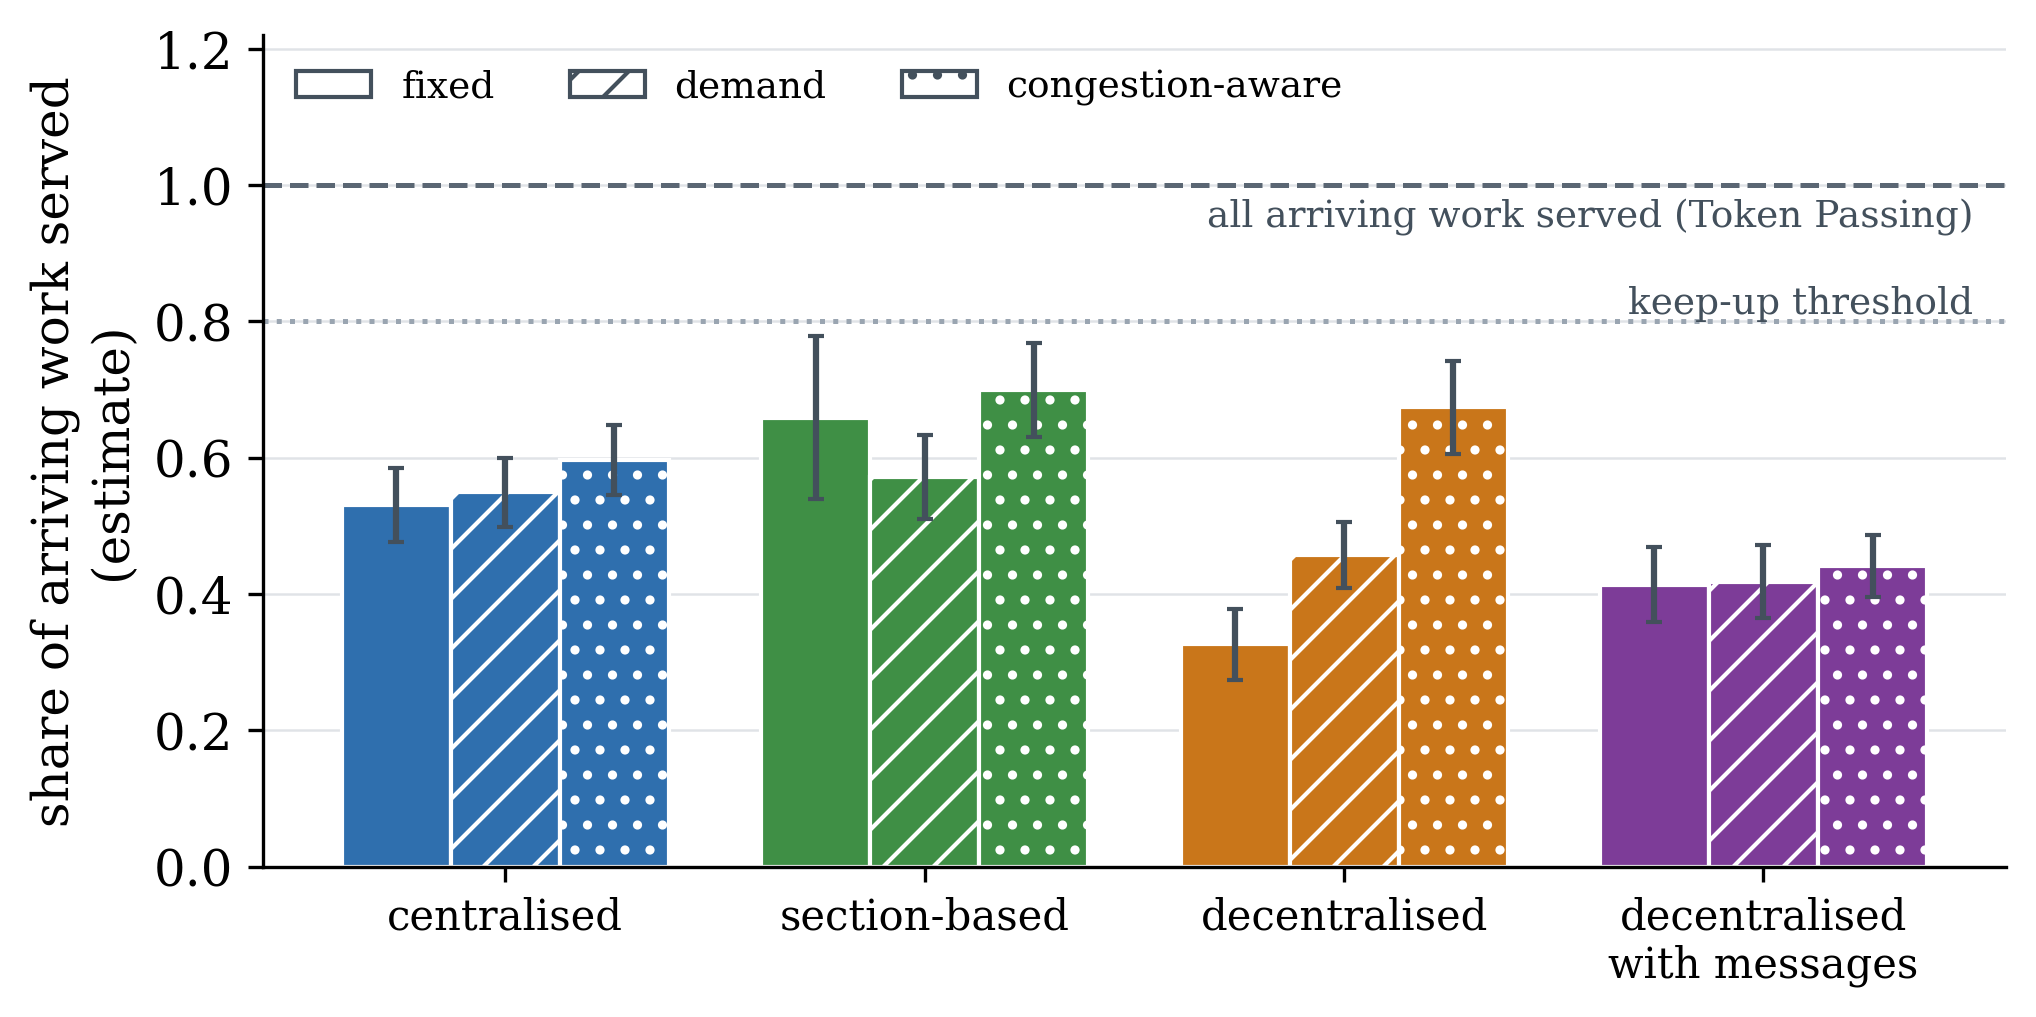
\includegraphics[width=0.85\linewidth]{results_fleet16/fleet16_served.png}
  \caption{\new{Share of the arriving work served on 16 agents, each rule with the policy trained under
  it, over 20 test seeds.}}
  \label{fig:app:throughput:16}
\end{figure}

\begin{figure}[h]
  \centering
  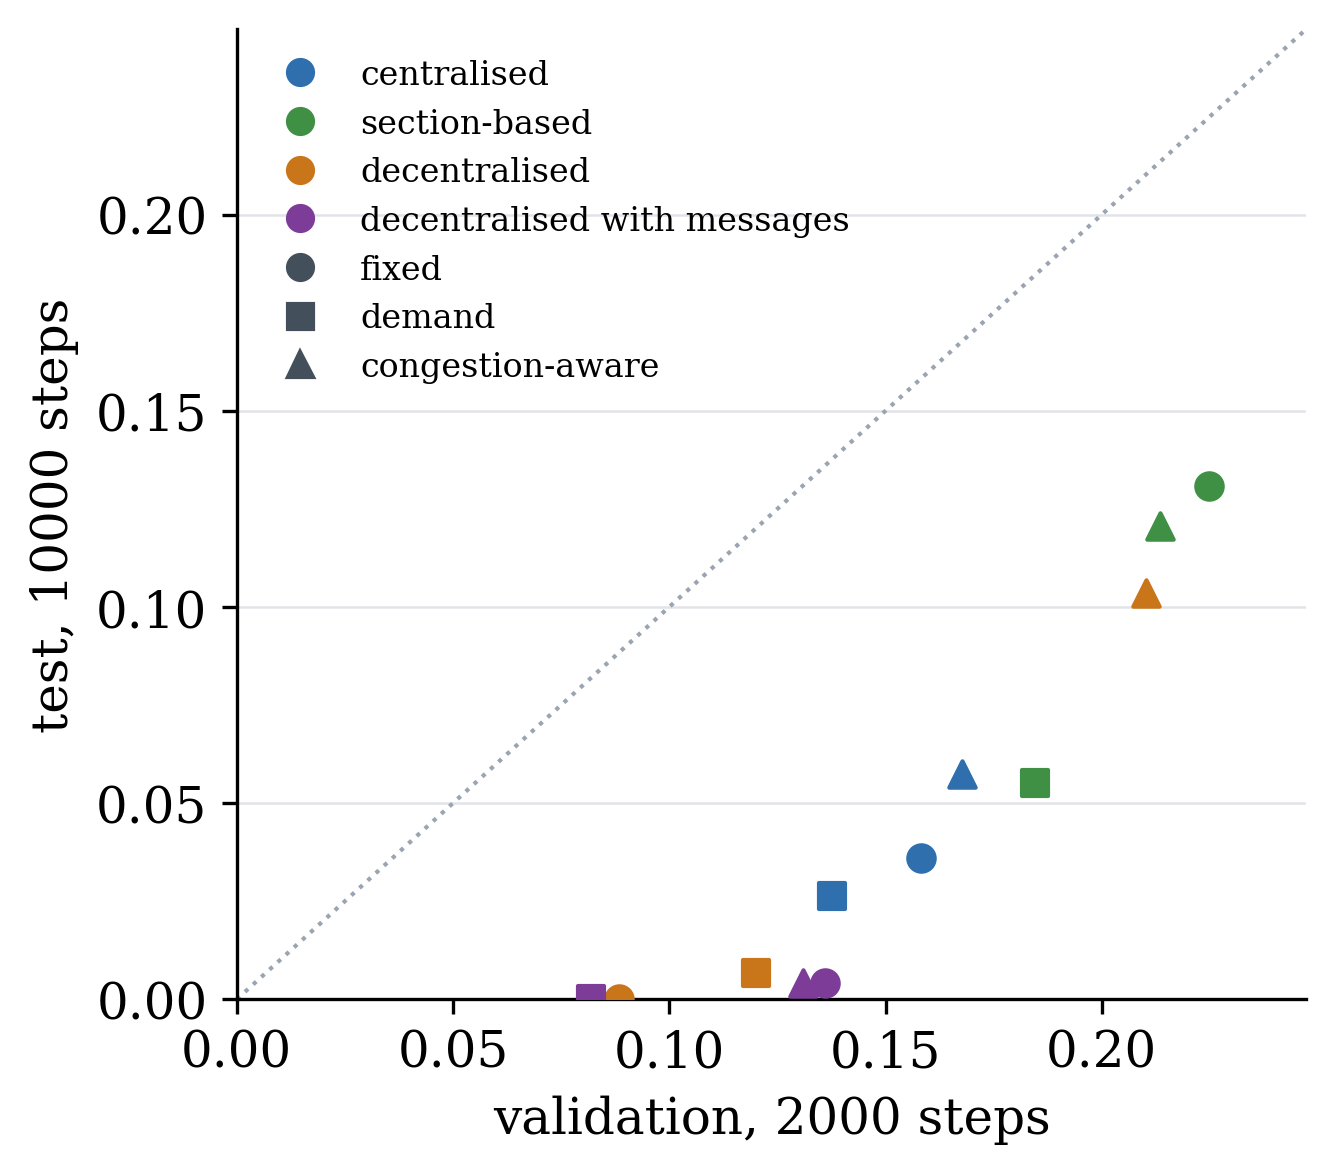
\includegraphics[width=0.5\linewidth]{results_fleet16/fleet16_val_vs_test.png}
  \caption{\new{Tasks done per step by each chosen policy, in the validation runs against the test
  runs, on 16 agents.}}
  \label{fig:app:valtest:16}
\end{figure}

\begin{figure}[h]
  \centering
  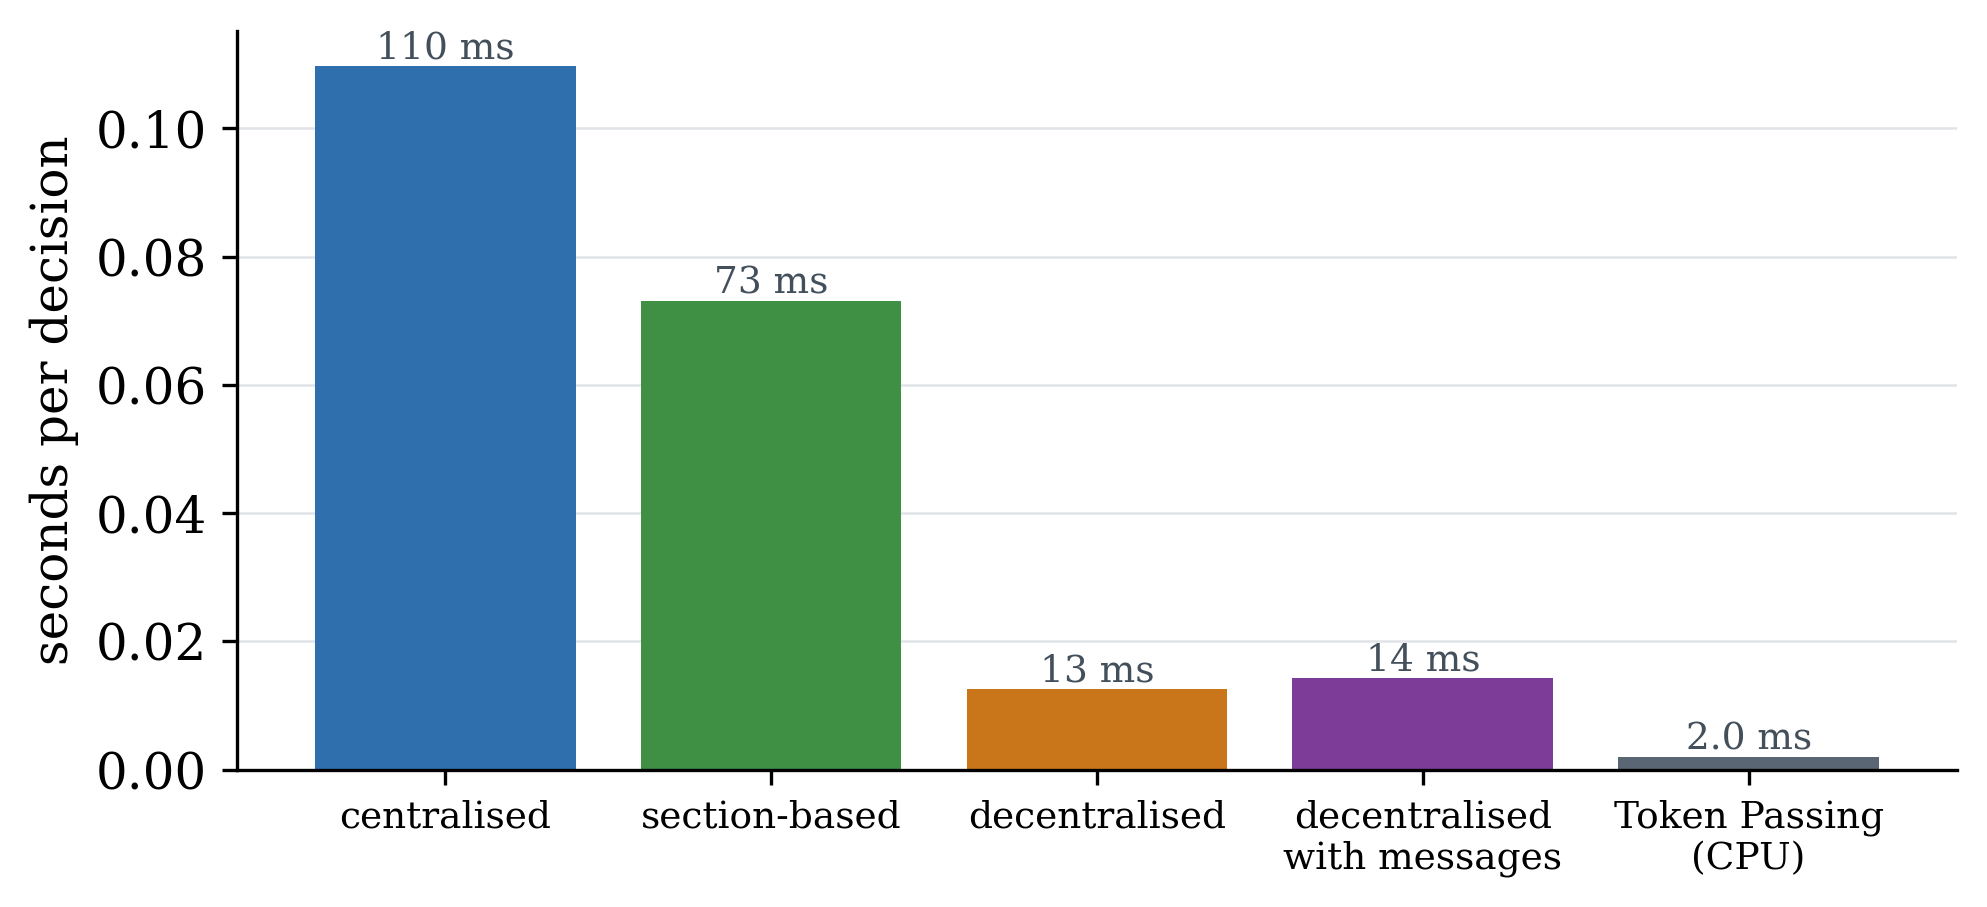
\includegraphics[width=0.75\linewidth]{results_fleet16/fleet16_runtime.png}
  \caption{\new{Mean decision time per step on 16 agents. The learned arms on the GPU, Token Passing
  on the CPU.}}
  \label{fig:app:runtime:16}
\end{figure}

\begin{table}[h]
  \centering
  \small
  \setlength{\tabcolsep}{4pt}
  \caption{\new{The keep-up check of the test runs on 16 agents, over 20 seeds.}}
  \label{tab:app:check:16}
  \begin{tabular}{llrrrrr}
    \toprule
    rule  &  controller  &  \shortstack{picks\\keep up}  &  \shortstack{put-aways\\keep up}  &  \shortstack{completed\\share}  &  \shortstack{backlog\\slope}  &  \shortstack{stalled\\runs} \\
    \midrule
    fixed      & Token Passing  & 20 of 20 & 20 of 20 & 0.98 & -0.05 & 0 \\
               & centralised    & 0 of 20 & 0 of 20 & 0.13 & 12.40 & 0 \\
               & section-based  & 2 of 20 & 1 of 20 & 0.45 & 9.02 & 0 \\
               & decentralised  & 0 of 20 & 0 of 20 & 0.00 & 17.82 & 0 \\
               & with messages  & 0 of 20 & 0 of 20 & 0.01 & 15.52 & 0 \\
    demand     & Token Passing  & 20 of 20 & 20 of 20 & 0.98 & 0.01 & 0 \\
               & centralised    & 0 of 20 & 0 of 20 & 0.09 & 12.80 & 0 \\
               & section-based  & 0 of 20 & 0 of 20 & 0.19 & 12.17 & 0 \\
               & decentralised  & 0 of 20 & 0 of 20 & 0.02 & 15.41 & 0 \\
               & with messages  & 0 of 20 & 0 of 20 & 0.00 & 16.53 & 0 \\
    congestion & Token Passing  & 20 of 20 & 20 of 20 & 0.98 & 0.01 & 0 \\
               & centralised    & 0 of 20 & 0 of 20 & 0.20 & 11.50 & 0 \\
               & section-based  & 0 of 20 & 0 of 20 & 0.41 & 8.59 & 0 \\
               & decentralised  & 0 of 20 & 0 of 20 & 0.36 & 9.31 & 0 \\
               & with messages  & 0 of 20 & 0 of 20 & 0.01 & 15.96 & 0 \\
    \bottomrule
  \end{tabular}
\end{table}

\begin{table}[h]
  \centering
  \small
  \setlength{\tabcolsep}{4pt}
  \caption{\new{The service time of picks and its parts in the test runs on 16 agents, as means over 20 seeds.}}
  \label{tab:app:result:16}
  \begin{tabular}{llrrrrrrrr}
    \toprule
    rule  &  controller  &  $\bar\zeta_T$  &  \shortstack{wait for\\agent}  &  travel  &  blocked  &  \shortstack{stock\\wait}  &  crowding  &  \shortstack{agents\\busy}  &  \shortstack{shelf\\taken} \\
    \midrule
    fixed      & Token Passing  & 126.5 & 105.4 & 19.5 & 1.5 & 0.02 & 0.06 & 0.40 & 35.4 \\
               & centralised    & 3655.0 & 3566.3 & 69.7 & 19.0 & 1157.63 & 0.14 & 1.00 & n/a \\
               & section-based  & 1377.5 & 1310.8 & 51.1 & 15.5 & 208.14 & 0.19 & 1.00 & n/a \\
               & decentralised  & n/a & n/a & n/a & n/a & n/a & 0.19 & 1.00 & n/a \\
               & with messages  & 4213.6 & 4135.1 & 54.9 & 23.6 & 1454.26 & 0.19 & 1.00 & n/a \\
    demand     & Token Passing  & 107.5 & 90.7 & 15.0 & 1.7 & 0.02 & 0.06 & 0.37 & 36.5 \\
               & centralised    & 3824.4 & 3731.1 & 70.7 & 22.6 & 1202.08 & 0.13 & 1.00 & n/a \\
               & section-based  & 3236.9 & 3151.9 & 59.3 & 25.7 & 963.29 & 0.16 & 1.00 & n/a \\
               & decentralised  & 4120.5 & 4058.2 & 48.1 & 14.2 & 1084.20 & 0.14 & 1.00 & n/a \\
               & with messages  & n/a & n/a & n/a & n/a & n/a & 0.20 & 1.00 & n/a \\
    congestion & Token Passing  & 108.2 & 91.4 & 15.2 & 1.6 & 0.02 & 0.06 & 0.37 & 35.7 \\
               & centralised    & 3350.2 & 3263.1 & 71.4 & 15.7 & 980.51 & 0.11 & 1.00 & n/a \\
               & section-based  & 2168.0 & 2096.1 & 58.5 & 13.4 & 505.47 & 0.13 & 1.00 & n/a \\
               & decentralised  & 2306.4 & 2225.8 & 60.7 & 19.9 & 546.28 & 0.15 & 1.00 & n/a \\
               & with messages  & 4273.7 & 4201.4 & 54.8 & 17.5 & 1257.26 & 0.17 & 1.00 & n/a \\
    \bottomrule
  \end{tabular}
\end{table}

\begin{table}[h]
  \centering
  \small
  \setlength{\tabcolsep}{4pt}
  \caption{\new{The cost and what the customer sees in the test runs on 16 agents, as means over 20 seeds.}}
  \label{tab:app:cost:16}
  \begin{tabular}{llrrrrrr}
    \toprule
    rule  &  controller  &  \shortstack{put-away\\service}  &  runtime $\kappa_T$  &  \shortstack{order\\completion}  &  \shortstack{orders\\per step}  &  $\Lambda_T$  &  $\Lambda_T/m$ \\
    \midrule
    fixed      & Token Passing  & 37.2 & 0.0019 & 256.4 & 0.033 & 0.265 & 0.0165 \\
               & centralised    & 3657.3 & 0.1095 & 2733.9 & 0.000 & 0.036 & 0.0022 \\
               & section-based  & 1394.0 & 0.0732 & 2712.6 & 0.009 & 0.131 & 0.0082 \\
               & decentralised  & n/a & 0.0113 & n/a & 0.000 & 0.000 & 0.0000 \\
               & with messages  & 4390.5 & 0.0146 & n/a & 0.000 & 0.004 & 0.0003 \\
    demand     & Token Passing  & 41.6 & 0.0020 & 208.2 & 0.034 & 0.284 & 0.0177 \\
               & centralised    & 3833.4 & 0.1098 & 4363.1 & 0.000 & 0.026 & 0.0017 \\
               & section-based  & 3239.5 & 0.0737 & 3698.9 & 0.001 & 0.055 & 0.0034 \\
               & decentralised  & 4134.2 & 0.0122 & n/a & 0.000 & 0.007 & 0.0004 \\
               & with messages  & n/a & 0.0138 & n/a & 0.000 & 0.000 & 0.0000 \\
    congestion & Token Passing  & 42.6 & 0.0020 & 207.8 & 0.034 & 0.285 & 0.0178 \\
               & centralised    & 3354.6 & 0.1100 & 3487.3 & 0.001 & 0.058 & 0.0036 \\
               & section-based  & 2188.0 & 0.0722 & 3348.8 & 0.005 & 0.121 & 0.0075 \\
               & decentralised  & 2303.9 & 0.0141 & 2930.1 & 0.004 & 0.104 & 0.0065 \\
               & with messages  & 4457.9 & 0.0144 & n/a & 0.000 & 0.004 & 0.0003 \\
    \bottomrule
  \end{tabular}
\end{table}

\begin{table}[h]
  \centering
  \small
  \setlength{\tabcolsep}{4pt}
  \caption{\new{What the backlog of the test runs on 16 agents is made of at the horizon, as means over 20 seeds.}}
  \label{tab:app:backlog:16}
  \begin{tabular}{llrrrrrr}
    \toprule
    rule  &  controller  &  \shortstack{waiting\\tasks}  &  \shortstack{active\\tasks}  &  \shortstack{waiting\\orders}  &  \shortstack{lines\\waited}  &  \shortstack{put-aways\\released}  &  \shortstack{put-aways\\done} \\
    \midrule
    fixed      & Token Passing  & 28.3 & 4.8 & 0.0 & 0.5 & 271.8 & 265.7 \\
               & centralised    & 598.2 & 11.0 & 535.5 & 798.6 & 261.1 & 34.4 \\
               & section-based  & 357.2 & 10.8 & 323.1 & 515.8 & 249.4 & 122.0 \\
               & decentralised  & 220.6 & 0.0 & 879.9 & 893.8 & 167.6 & 0.0 \\
               & with messages  & 448.6 & 2.1 & 744.5 & 863.9 & 225.3 & 4.3 \\
    demand     & Token Passing  & 26.4 & 4.7 & 0.0 & 1.0 & 271.8 & 265.4 \\
               & centralised    & 593.2 & 8.8 & 579.7 & 823.7 & 257.8 & 25.6 \\
               & section-based  & 543.2 & 11.1 & 501.7 & 764.4 & 257.1 & 51.2 \\
               & decentralised  & 428.6 & 2.6 & 757.0 & 863.3 & 228.1 & 6.8 \\
               & with messages  & 278.8 & 0.0 & 854.8 & 891.5 & 183.1 & 0.0 \\
    congestion & Token Passing  & 25.9 & 4.8 & 0.0 & 0.8 & 271.8 & 265.7 \\
               & centralised    & 617.5 & 12.7 & 449.4 & 754.1 & 269.8 & 54.1 \\
               & section-based  & 522.7 & 13.4 & 278.9 & 582.7 & 271.8 & 110.9 \\
               & decentralised  & 533.4 & 12.7 & 336.4 & 623.6 & 269.6 & 95.0 \\
               & with messages  & 414.8 & 2.3 & 764.0 & 864.9 & 218.1 & 4.5 \\
    \bottomrule
  \end{tabular}
\end{table}


\subsection*{\new{Appendix L, ``The same policy under each rule''}}

\new{Each arm's policy trained under fixed storage was also played under demand and congestion-aware
storage. The policy stays the same, so any change comes from the storage rule alone. The test is the
same as above, 20 seeds of 10000 steps with the first 5000 left out.}

\new{The storage rule on its own changes nothing the test can measure
(Table~\ref{tab:app:regime1:16}). Under congestion-aware storage the centralised and section-based
arms each finish 0.002 fewer tasks per step than under fixed storage. Compared seed by seed, the
95\,\% interval holds zero for both. The rule does better on only 5 and 6 of the 20 seeds. The agents
crowd a little less (0.19 against 0.18 for the section-based arm) and stand blocked a little less, but
these gaps are inside the noise too.}

\new{The better congestion-aware rows of the tables above come from the training run, not from
storage. Under the same rule, the decentralised policy trained under congestion-aware storage
finishes 0.104 tasks per step, and the one trained under fixed storage finishes none. For the
centralised arm it is 0.058 against 0.034. Both do better on 16 of the 20 seeds. The section-based
arm and the arm with messages do not change. Each arm has one training run per rule, so this cannot
tell training under the rule apart from a better training run. The decentralised run trained under
fixed storage was already weak in validation, at 0.088 tasks per step against 0.210.}

\new{Two arms show nothing about storage here. The decentralised policy and the policy with messages
trained under fixed storage finish almost no picks under any rule, so there is no effect for the rule
to change.}

\new{Whether any of these runs keeps up waits for the replay with the served share. The tasks per step
do not depend on that check.}

\begin{table}[h]
  \centering
  \small
  \setlength{\tabcolsep}{4pt}
  \caption{\new{Tasks done per step on 16 agents, the fixed-trained policy under each rule, means over
  20 seeds. The last column is the policy trained under congestion-aware storage.}}
  \label{tab:app:regime1:16}
  \begin{tabular}{lrrrrr}
    \toprule
    controller & fixed & demand & \shortstack{congestion-\\aware} & \shortstack{difference to fixed\\{[95\,\% interval]}} & \shortstack{own policy,\\congestion-aware} \\
    \midrule
    centralised    & 0.036 & 0.035 & 0.034 & $-0.002$ [$-0.008$, 0.004] & 0.058 \\
    section-based  & 0.131 & 0.125 & 0.129 & $-0.002$ [$-0.015$, 0.012] & 0.121 \\
    decentralised  & 0.000 & 0.000 & 0.000 & 0.000 & 0.104 \\
    with messages  & 0.004 & 0.003 & 0.000 & $-0.004$ [$-0.011$, 0.003] & 0.004 \\
    \bottomrule
  \end{tabular}
\end{table}

\subsection*{Appendix L, ``Stock in the test runs''}

\begin{table}[h]
  \centering
  \small
  \setlength{\tabcolsep}{4pt}
  \caption{\new{How the stock is spread and how old it is when picked, at the main load on 16 agents, as means over 20 seeds.}}
  \label{tab:app:stock:16}
  \begin{tabular}{llrrrrrr}
    \toprule
    rule  &  controller  &  \shortstack{split\\SKUs}  &  \shortstack{tasks\\per line}  &  \shortstack{old stock\\on prime}  &  \shortstack{unit age\\at pick}  &  updates  &  \shortstack{arrived\\units} \\
    \midrule
    fixed      & Token Passing  & 31.5 & 1.03 & 0.27 & 1179 & 100 & 51.7 \\
               & centralised    & 25.5 & 1.15 & 0.30 & 2476 & 100 & 51.6 \\
               & section-based  & 26.3 & 1.12 & 0.31 & 1961 & 100 & 51.6 \\
               & decentralised  & 19.1 & 1.04 & 0.30 & 3444 & 100 & 51.6 \\
               & with messages  & 22.8 & 1.12 & 0.31 & 3011 & 100 & 51.6 \\
    demand     & Token Passing  & 35.5 & 1.14 & 0.39 & 1098 & 100 & 51.7 \\
               & centralised    & 31.1 & 1.16 & 0.30 & 2561 & 100 & 51.6 \\
               & section-based  & 31.9 & 1.16 & 0.32 & 2460 & 100 & 51.6 \\
               & decentralised  & 28.3 & 1.12 & 0.31 & 3027 & 100 & 51.6 \\
               & with messages  & 21.8 & 1.09 & 0.31 & 3598 & 100 & 51.6 \\
    congestion & Token Passing  & 35.5 & 1.14 & 0.37 & 1107 & 100 & 51.7 \\
               & centralised    & 32.5 & 1.18 & 0.26 & 2315 & 100 & 51.6 \\
               & section-based  & 33.3 & 1.18 & 0.27 & 2052 & 100 & 51.6 \\
               & decentralised  & 33.0 & 1.18 & 0.25 & 2158 & 100 & 51.6 \\
               & with messages  & 27.8 & 1.13 & 0.26 & 2980 & 100 & 51.6 \\
    \bottomrule
  \end{tabular}
\end{table}

\section*{Part 3. Questions}

\begin{enumerate}[leftmargin=1.4em]
\item The shares in the figure are estimated from the backlog slope until the replay is home
  ([A96], open point 2). The keep-up table then uses the new check.
\item \new{Regime 1 is added as its own subsection (version 3). Keep it in Appendix~L, or also give its
  main point, that the storage rule alone changes nothing at 16 agents, one sentence in the results
  chapter?}
\item The figures in Appendix~L, or only the tables, with the figures in the Experiments chapter
  later?
\item The pick service time and its parts (Table~\ref{tab:app:result:16}) grow with the length of a
  run that falls behind. Keep them as they are, or show ``n/a'' for a rule where no seed keeps up?
\item Fleet 8 is not filled yet. The centralised fixed test is stuck on Kaggle. Fill fleet 8 once it is
  home, in the same form?
\end{enumerate}

\end{document}
